\documentclass[a4paper, 11pt]{article}
\usepackage[utf8]{inputenc}
\usepackage[T1]{fontenc}
\usepackage{lmodern}
\usepackage[margin=1in]{geometry}
\usepackage{amsmath, amssymb}
\usepackage{booktabs}
\usepackage[protrusion=true,expansion=false]{microtype}
\usepackage{xcolor}
\usepackage{listings}
\usepackage{tcolorbox}
\usepackage{url}
\usepackage{graphicx}

% Color scheme
\definecolor{codegreen}{rgb}{0.15, 0.55, 0.15}
\definecolor{codegray}{rgb}{0.45, 0.45, 0.45}
\definecolor{codeblue}{rgb}{0.12, 0.35, 0.75}
\definecolor{backcolour}{rgb}{0.96, 0.97, 0.98}
\definecolor{termbg}{rgb}{0.14, 0.15, 0.17}
\definecolor{termfg}{rgb}{0.92, 0.92, 0.92}

% Code snippet styling
\lstdefinestyle{erlstyle}{
    backgroundcolor=\color{backcolour},   
    commentstyle=\color{codegreen}\itshape,
    keywordstyle=\color{codeblue}\bfseries,
    numberstyle=\tiny\color{codegray},
    stringstyle=\color{codegray},
    basicstyle=\ttfamily\footnotesize,
    breaklines=true,                 
    keepspaces=true,                 
    tabsize=2,
    frame=single,
    rulecolor=\color{black!10}
}
\lstset{style=erlstyle}

% Terminal trace box styling
\tcbset{
    terminalbox/.style={
        colback=termbg,
        colupper=termfg,
        colframe=black!65,
        arc=3pt,
        boxrule=1pt,
        fontupper=\ttfamily\footnotesize,
        left=6pt, right=6pt, top=5pt, bottom=5pt
    }
}

\title{\textbf{Report 2: Routy}}
\author{\textbf{Rodrigo Perestrelo, Lennard Last} \\ ID2201 Distributed Systems, Basic Course}
\date{\today{}}

\begin{document}

\maketitle

\section{Introduction}

The objective of this assignment is to design, implement, and empirically evaluate a decentralized link-state routing protocol. This protocol requires every router to independently construct an identical global graph of the network topology and locally compute optimal next-hop forwarding paths using Dijkstra's algorithm.

\section{What Was Difficult and How It Was Solved}

\subsection{Implementing Dijkstra's Algorithm and Routing Table Construction}
\textbf{The Problem:} Implementing Dijkstra's algorithm in a purely functional language required iteratively relaxing paths while keeping track of the direct next-hop gateway for every destination.

\textbf{The Solution:} In \texttt{update/4}, we check whether a node already exists in the sorted list via \texttt{entry/2}. If absent (returning \texttt{0}), it has already been settled and is safely discarded. If present with a greater distance, it is replaced with the shorter path and the corresponding gateway:

\begin{lstlisting}[language=erlang]
update(Node, N, Gateway, Sorted) ->
    case entry(Node, Sorted) of
        0 -> Sorted;
        Length when Length > N ->
            replace(Node, N, Gateway, Sorted);
        Length when Length =< N ->
            Sorted
    end.
\end{lstlisting}

\noindent During table generation in \texttt{iterate/3}, the node with the minimal distance is extracted from the sorted list, committed to the final routing table as \texttt{\{Dest, Gateway\}}, and its adjacent links from \texttt{Map} are relaxed using \texttt{update/4} before recursing.

\subsection{Preventing Broadcast Storms and Stale LSAs in Cyclic Networks}
\textbf{The Problem:} Link-state advertisements flooded over cyclic topologies will loop indefinitely if routers lack memory of forwarded packets, causing broadcast storms and packet duplication.

\textbf{The Solution:} In \texttt{hist.erl}, each router tags advertisements with an incrementing integer sequence counter $N$. A received message from router $Node$ with sequence number $R$ is discarded as \texttt{old} if $R \le \text{Counter}$. Furthermore, by initializing a router's own identity as $\{Name, \text{inf}\}$, any self-generated message that cycles back through the network is rejected:
\begin{lstlisting}[language=erlang]
update(Node, N, History) ->
    case lists:keyfind(Node, 1, History) of
        false -> {new, [{Node, N} | History]};
        {Node, Counter} when Counter < N ->
            NewHist = lists:keydelete(Node, 1, History),
            {new, [{Node, N} | NewHist]};
        {Node, Counter} when Counter >= N -> old
    end.
\end{lstlisting}

\subsection{Solved Improvement: Autonomous Event-Driven Convergence}
\textbf{The Problem:} In the base specification, link-state flooding (\texttt{broadcast}) and path recomputation (\texttt{update}) required manual invocation via external console messages whenever a network event occurred.

\textbf{The Solution:} We eliminated manual steps by integrating autonomous reactive flooding directly into \texttt{routy.erl}. When a router traps a \texttt{'DOWN'} process exit, or executes an \texttt{add} or \texttt{remove} interface mutation, it increments sequence counter $N$, immediately broadcasts its updated interface list to all direct peers via \texttt{intf:broadcast/2}, and recomputes its table. Furthermore, upon receiving a novel link-state advertisement (\texttt{\{links, ...\}}), routers automatically update their graph and recalculate their Dijkstra table on the fly:

\begin{lstlisting}[language=erlang]
{'DOWN', Ref, process, _, _} ->
    {ok, Down} = intf:name(Ref, Intf),
    io:format("~w: exit recived from ~w~n", [Name, Down]),
    Intf1 = intf:remove(Down, Intf),
    Message = {links, Name, N, intf:list(Intf1)},
    intf:broadcast(Message, Intf1),
    Table1 = dijkstra:table(intf:list(Intf1), Map),
    router(Name, N+1, Hist, Intf1, Table1, Map);
{links, Node, R, Links} ->
    case hist:update(Node, R, Hist) of
        {new, Hist1} ->
            intf:broadcast({links, Node, R, Links}, Intf),
            Map1 = map:update(Node, Links, Map),
            Table1 = dijkstra:table(intf:list(Intf), Map1),
            router(Name, N, Hist1, Intf, Table1, Map1);
        old ->
            router(Name, N, Hist, Intf, Table, Map)
    end;
\end{lstlisting}

\section{Remaining Potential Improvements to Routy}

\begin{enumerate}
    \item \textbf{Weighted Edge Costs:} The protocol currently assumes unit link costs (hop count). Incorporating latency or bandwidth metrics into \texttt{map.erl} would allow Dijkstra to select throughput-optimal paths across diverse physical connections.
    \item \textbf{LSA Garbage Collection:} The history tracking list in \texttt{hist.erl} grows indefinitely as new nodes are discovered. Implementing a time-to-live (TTL) on history records would prevent unbounded memory growth in long-running networks.
\end{enumerate}

\section{Automated Testing and Bonus Evaluation: The World}

To evaluate Routy's end-to-end performance and autonomous fault recovery, we implemented a 14-node European network harness (\texttt{world\_test.erl}) interconnecting major transit centers across Scandinavia, Central Europe, and the Iberian Peninsula.

\begin{figure}[htbp]
\centering
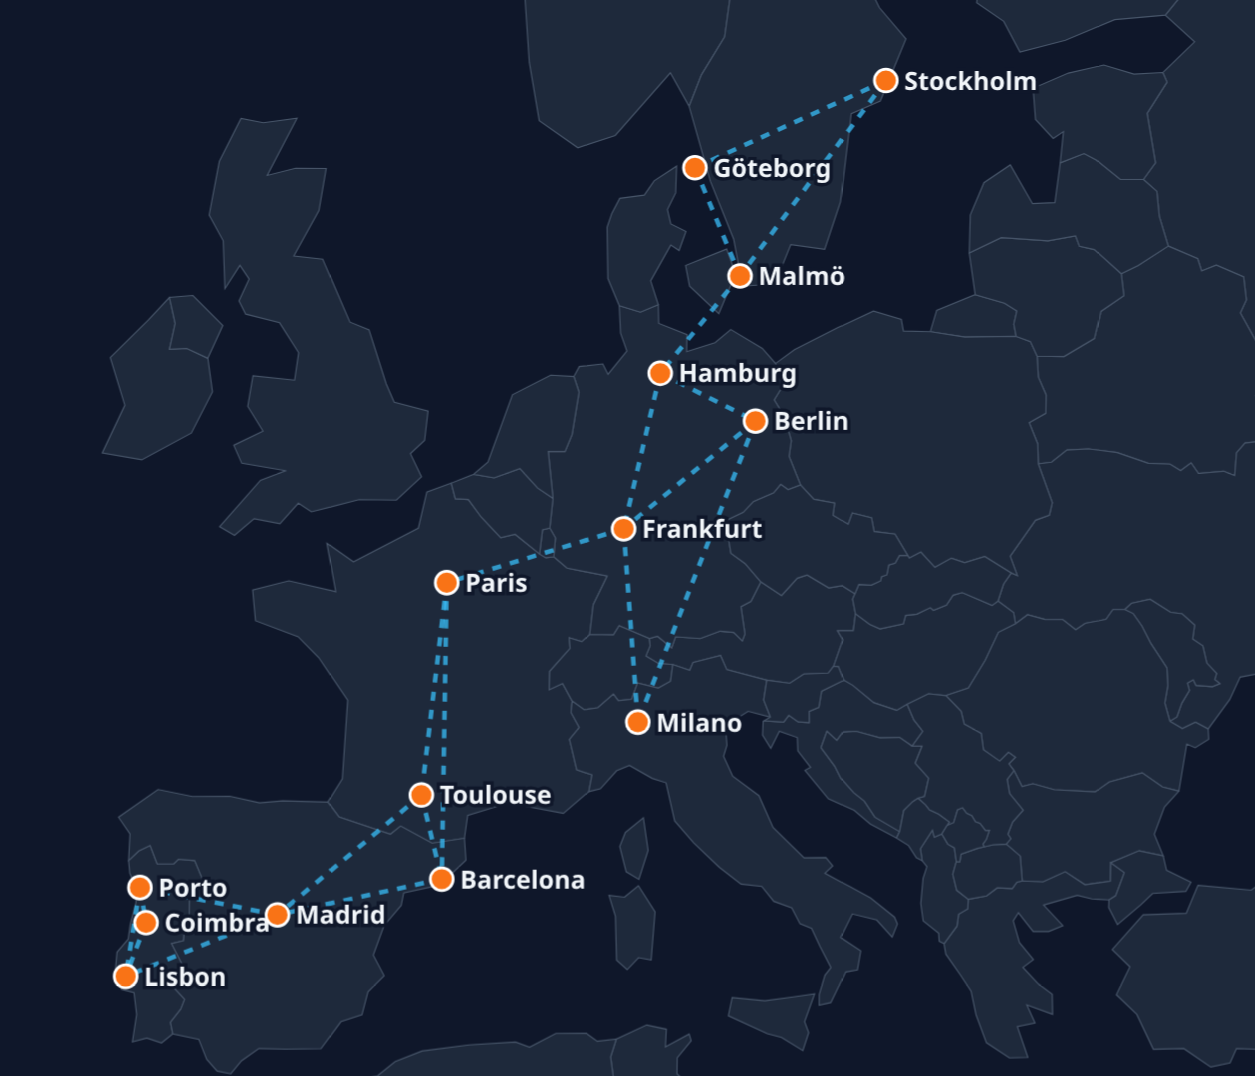
\includegraphics[width=0.65\textwidth]{world_map.png}
\caption{Topology of the 14-node network harness. Multi-homed connections provide redundancy across the Iberian and Central European corridors.}
\label{fig:world_map}
\end{figure}

\subsection{Can we send messages across distant nodes in the topology?}
\textbf{Yes.} Once initial interface advertisements flooded through the network and Dijkstra tables converged, multi-hop routing succeeded across the continent from Stockholm to Lisbon:
\begin{tcolorbox}[terminalbox]
1> world\_test:route\_message(stockholm, lisbon, ola). \\
routing message: "ola" \\
from: stockholm $\rightarrow$ to: lisbon \\
stockholm: routing message ("ola") \\
malmo: routing message ("ola") \\
hamburg: routing message ("ola") \\
frankfurt: routing message ("ola") \\
paris: routing message ("ola") \\
barcelona: routing message ("ola") \\
madrid: routing message ("ola") \\
lisbon: received message "ola"
\end{tcolorbox}
\noindent The computed primary shortest path traverses 7 intermediate hops:
$$\text{stockholm} \rightarrow \text{malmo} \rightarrow \text{hamburg} \rightarrow \text{frankfurt} \rightarrow \text{paris} \rightarrow \text{barcelona} \rightarrow \text{madrid} \rightarrow \text{lisbon}$$

\subsection{Will routing functionality still work if we stop routers or close nodes?}
\textbf{Yes}, provided an alternate physical path exists in the topology.

We halted the critical Iberian junction router Barcelona (\texttt{r10}) using \texttt{world\_test:kill\_router(barcelona)}. Its monitored peers (\texttt{paris}, \texttt{madrid}, and \texttt{toulouse}) caught the termination exit immediately:
\begin{tcolorbox}[terminalbox]
paris: exit recived from barcelona \\
stop \\
madrid: exit recived from barcelona \\
toulouse: exit recived from barcelona
\end{tcolorbox}

Thanks to our autonomous re-convergence enhancement, the surviving neighbors automatically broadcast their updated interface lists and recomputed their tables without manual console commands. Dispatching another message from Stockholm to Lisbon succeeded, dynamically routing around the dead Barcelona node via Toulouse:
\begin{tcolorbox}[terminalbox]
3> world\_test:route\_message(stockholm, lisbon, ola). \\
routing message: "ola" \\
from: stockholm $\rightarrow$ to: lisbon \\
stockholm: routing message ("ola") \\
malmo: routing message ("ola") \\
hamburg: routing message ("ola") \\
frankfurt: routing message ("ola") \\
paris: routing message ("ola") \\
toulouse: routing message ("ola") \\
madrid: routing message ("ola") \\
lisbon: received message "ola"
\end{tcolorbox}

\subsection{How long between a disabled network card and the delivery of a 'DOWN' message?}
The detection latency depends directly on the failure mechanism:
\begin{itemize}
    \item \textbf{Router Process Crash or Shell Exit (\texttt{q().}):} Takes \textbf{$< 2$ ms} to \textbf{$< 15$ ms}. When a process dies or an OS terminates the VM, the operating system kernel closes open TCP sockets immediately with a \texttt{FIN} or \texttt{RST} packet. The remote Erlang runtime traps this socket closure instantly.
    \item \textbf{Disabled Network Interface / Pulled Cable:} Takes \textbf{45 to 60 seconds}. When a physical link is severed, no TCP teardown packets are transmitted. Surviving nodes cannot distinguish an idle connection from a dead interface. The runtime must wait for Erlang's distribution heartbeat timer (\texttt{net\_ticktime}, default 60 seconds) to expire before flagging the node as unreachable and dispatching the \texttt{'DOWN'} message.
\end{itemize}

\section{Conclusions}

This laboratory demonstrated the separation between the control plane (graph flooding and shortest-path computation) and the data plane (packet forwarding). Erlang's lightweight actor model, process monitors, and pattern matching provided clean abstractions for implementing link-state protocols. Integrating autonomous event-driven flooding eliminated the need for manual intervention, enabling self-healing network behavior upon node failure.

\end{document}